\scanpage{200}
\mspage{399}

\[
\begin{aligned}
(79)\qquad u_{\alpha,\beta,f}
&\overset{\mathrm{dfn}}{=}f^{-1}u_{\alpha,\beta}
=(\mu\delta)\overbrace{f^{-1}\alpha}^{\alpha_0}(c\rho+d)=\\
&=\mu\underbrace{f^{-1}\beta}_{\beta_0}(t\sigma_\infty+u)\tau_\infty^{\alpha_2}
\end{aligned}
\]
and one finds, as one should,
\[
(80)\qquad
\left\{\begin{aligned}
u_{\alpha,\beta,f}(\sigma_\infty)&=\operatorname{int}(\beta_0)(\sigma_\infty)\\
u_{\alpha,\beta,f}(\rho)&=\operatorname{int}(\unsure{\alpha_0|\beta_0})(\rho)
\end{aligned}\right.,
\]
\margin{\figure{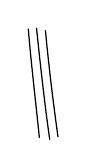
\begin{tikzpicture}[x=1mm,y=1mm,line width=.45pt,line cap=round]
\draw (0,14.0) .. controls (.36,9.6) and (1.02,4.1) .. (1.40,.25);
\draw (1.05,14.1) .. controls (1.53,9.4) and (2.14,4.0) .. (2.72,0);
\draw (2.18,13.8) .. controls (2.62,9.0) and (3.26,4.0) .. (3.77,.32);
\end{tikzpicture}}}
\margin{\uline{N.B.} \unsure{if|If} $u,\sigma$ are elements of a group $G$, one of course sets $u(\sigma)=u\sigma u^{-1}$.}
\margin{this \uline{implies that}, \deleted{\unsure{by}} $\operatorname{int}(u_{\alpha,\beta,f})$ has the same effect, \unsure{on|in} $\mathrm{Sl}(2,\widehat{\mathbb Z})'$ as the \unsure{automorphism} $u$ of $\unsure{\widehat{\mathcal G}_{0,3}^{+}|\widetilde{\mathcal G}_{0,3}^{\to}}$ defined (when there is one), by passage to the quotient in $\mathrm{Sl}(2,\widehat{\mathbb Z})'$.}

formulas which reduce to formulas in which $f$ has again disappeared
\[
(81)\qquad
\left\{\begin{aligned}
u_{\alpha,\beta}(\sigma_\infty)&=\operatorname{int}(\beta)(\sigma_\infty)\\
u_{\alpha,\beta}(\rho)&=\operatorname{int}(\unsure{\alpha|\beta})(\rho)
\end{aligned}\right.,
\]
which \deleted{in turn} follow \inserted{\uline{trivially}} from the two expressions \deleted{of} (78) for $u_{\alpha,\beta}$!

The formulas (80) are naturally completed by
\[
(82)\qquad
u_{\alpha,\beta,f}(\varepsilon_0)
=\deleted{\unsure{f\varepsilon_0}}\inserted{\varepsilon}\operatorname{int}(f^{-1})(\varepsilon_0^\mu)
\qquad\deleted{\unsure{(\varepsilon=\varepsilon_2)}}
\]
\[
(\text{where }\varepsilon=\varepsilon_2\in\{\pm1\})
\]
\margin{\figure{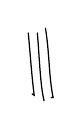
\begin{tikzpicture}[x=1mm,y=1mm,line width=.45pt,line cap=round]
\draw (0,8.6) .. controls (.28,5.5) and (.48,2.7) .. (.75,.7) -- (.48,.86);
\draw (1.15,8.6) .. controls (1.44,5.1) and (1.52,2.0) .. (2.0,0);
\draw (2.18,9.2) .. controls (2.68,6.2) and (2.62,2.9) .. (3.15,.43) -- (2.90,.39);
\end{tikzpicture}}}
which in turn reduces to
\[
(83)\qquad u_{\alpha,\beta}(\varepsilon_0)=\varepsilon.\varepsilon_0^\mu
\]
where $f$ no longer appears. Since $\varepsilon_0=\sigma_\infty\rho$, this formula reduces to:
\[
u_{\alpha,\beta}(\sigma_\infty)u_{\alpha,\beta}(\rho)=\varepsilon.\varepsilon_0^\mu,
\]
which in view of (81) reduces to:
\[
\operatorname{int}(\beta)(\sigma_\infty)\operatorname{int}(\unsure{\alpha|\beta})(\rho)=\varepsilon.\varepsilon_0^\mu
\]
\deleted{\unsure{then}}
\[
\deleted{\unsure{\alpha\sigma_\infty\alpha^{-1}\beta\rho\beta^{-1}}}
\]

\scanpage{201}

now the first \unsure{side} is written
\[
\deleted{\unsure{\beta\sigma_\infty\beta^{-1}\alpha\rho\alpha^{-1}
=(\beta\sigma_\infty\beta^{-1}\sigma_\infty)(\sigma_\infty\rho)(\rho^{-1}\alpha\rho\alpha^{-1})}}
\]
\[
\deleted{\unsure{=(\beta\sigma_\infty(\beta)^{-1})\varepsilon_0(\rho^{-1}(\alpha)\beta^{-1})}}
\]
\[
\begin{aligned}
\beta\sigma_\infty\beta^{-1}\alpha\rho\alpha^{-1}
&=\underbrace{(\beta\sigma_\infty\beta^{-1}\sigma_\infty)}_{\beta\sigma_\infty(\beta)^{-1}}
\underbrace{(\sigma_\infty\rho)}_{\varepsilon_0}
\underbrace{(\rho^{-1}\alpha\rho\alpha^{-1})}_{\rho^{-1}(\alpha)\alpha^{-1}=\rho^{-1}(\alpha\rho(\alpha)^{-1})}\\
&=\eta.\varepsilon_0.\rho^{-1}(\xi)
=\eta.\underbrace{(\varepsilon_0\rho^{-1})}_{\sigma_\infty}(\xi).\varepsilon_0
=\eta\sigma_\infty(\xi)\varepsilon_0
\end{aligned}
\]
so relation (83) is also written
\[
\eta\sigma_\infty(\xi)=\varepsilon\varepsilon_0^{\mu-1}\quad(=\varepsilon \ell_0^\nu)
\]
now one has $\xi=\varepsilon\eta \ell_1^\nu$ (loop relation (60))

so
\[
\eta\sigma_\infty(\xi)=\varepsilon\eta\sigma_\infty(\eta)\ell_0^\nu=\varepsilon \ell_0^\nu,\quad\text{OK.}
\]

\uline{Remark.} All these formulas are valid in $\mathrm{Gl}(2,\widehat{\mathbb Z})$, without ambiguity of signs, once $\alpha,\beta,f$ are chosen. If one changes the signs of $\alpha$ \unsure{or|and} of $\beta$ or both, the loop relation is not modified --- and $u_{\alpha,\beta}$ is not \unsure{changed} either, \deleted{On the other hand} nor $u_{\alpha,\beta,f}$ (if one does not touch $f$). On the other hand, a \unsure{change} of sign on $f$ implies a \unsure{change} of sign on $u_{\alpha,\beta,f}$. But such a change of sign of course changes nothing as to the validity of formulas (80), (82). When one makes

\scanpage{202}
\mspage{400}

on $(\alpha,\beta,f)$ the changes \unsure{the}
\[
(84)\qquad
\alpha'=\ell_0^n\alpha,\qquad\beta'=\ell_0^n\beta,\qquad f'=\ell_0^n f
\qquad(n\in\mathbb Z)
\]
then \deleted{\illegible{1}}
\[
(85)\qquad
\left\{\begin{aligned}
c'&=\unsure{c},\quad d'=d& t'&=t,\quad u'=u\\
\underbrace{f'^{-1}\alpha'}_{\alpha'_0}&=\underbrace{f^{-1}\alpha}_{\alpha_0}&
\underbrace{f'^{-1}\beta'}_{\beta'_0}&=\underbrace{f^{-1}\beta}_{\beta_0}
\end{aligned}\right.
\qquad\deleted{\unsure{\mu'=\mu|u'=u}}
\]
\deleted{finally}
\[
\deleted{\unsure{\delta'=\delta}\text{ since}}
\qquad\deleted{\unsure{u_{\alpha',\beta'}}}
\]
finally
\[
\delta'(=\det\alpha')=\delta(=\det\alpha)\quad(\text{since }\det \ell_0^n=1)
\]
\[
(86)\qquad
\left\{\begin{aligned}
\text{hence}\quad\deleted{\unsure{f}}\quad
\mu'\bigl(=\delta'/(c'^2+c'd'+d'^2)\bigr)&=\mu\bigl(=\delta/(c^2+cd+d^2)\bigr)\\
\text{hence}\quad\varepsilon'_2&=\varepsilon_2,\quad\alpha'_2=\alpha_2.
\end{aligned}\right.
\]
this is \unsure{twice} what is needed to check \inserted{with (79)} that
\[
(87)\qquad u_{\alpha',\beta',f'}=u_{\alpha,\beta,f}.
\]

Let us also recall (cf. proposition page 384)

\uline{Proposition.} Let $\mu\in\widehat{\mathbb Z}^*$, hence the signs $\varepsilon_2=\varepsilon_2(\mu)$ and $\varepsilon_3=\varepsilon_3(\mu)$ (defined by $\mu\equiv\varepsilon_2\ (4)$, $\mu\equiv\varepsilon_3\ (3)$), and let $c,d,t,u\in\widehat{\mathbb Z}$. For there to exist $a,b,r,s\in\widehat{\mathbb Z}$
\[
\alpha=\begin{pmatrix}a&b\\c&d\end{pmatrix},\qquad
\beta=\begin{pmatrix}r&s\\t&u\end{pmatrix}
\quad\text{satisfying (64)}
\]
\[
ad-bc=\varepsilon_3\qquad ru-st=1
\]
and the loop relation
\[
\alpha\rho(\alpha)^{-1}=\varepsilon_2\bigl(\beta\sigma_\infty(\beta^{-1})\bigr)\ell_1^\nu
\qquad\text{where }\nu=(\mu-1)/2
\]
(i.e. relations (73)) it is necessary and sufficient that one have
\[
(88)\qquad\varepsilon_3(c^2+cd+d^2)=\varepsilon_2(t^2+u^2)=1/\mu,
\]
and \unsure{the set|the set} of pairs $(\alpha,\beta)$ satisfying these conditions is a \uline{torsor} under $\widehat{\mathbb Z}$, operating

\margin{\uline{N.B.} For fixed $\mu$, one can always find $c,d,t,u$ satisfying relation (88) --- fortunately!}

\scanpage{203}

by
\[
 (\alpha,\beta)\longmapsto
 (\unsure{\varepsilon_0^n}\alpha,\varepsilon_0^n\beta).
\]
\deleted{\illegible{1}}

\uline{Corollary} For one to be able to find $\alpha,\beta$ such that one has in addition $\alpha\equiv\beta\equiv1\ (2)$, it is necessary and sufficient that one have
\[
\tag{89}
 c\equiv t\equiv0\ (2)\qquad d\equiv u\equiv\unsure{1}\ (2),
\]
and then \unsure{the set} of solutions $(\alpha,\beta)$ satisfying these additional conditions is a torsor under $\widehat{\mathbb Z}$, operating by
\[
 (\alpha,\beta)\longmapsto(\ell_0^n\alpha,\ell_0^n\beta).
\]

\uline{Scholium} One can thus say that for an element \inserted{$u$} of $\mathcal N_{0,3}^{!\sim}$, which defines \unsure{thus|two} $\alpha,\beta$ in $\Pi_{0,3}^{\sim\wedge},\Pi_{0,3}^{\wedge}$ \inserted{(\uline{modulo} the \unsure{transformations} $(\alpha,\beta)\mapsto(\ell_0^n\alpha,\ell_0^n\beta)$),} (satisfying the loop relation), there are attached to it the ``adelic invariants'' \deleted{\illegible{3}}
\[
\tag{90}
 \Theta=(\mu,c,d,t,u)
\]
($c,d,t,u$ determined up to \unsure{\uline{ambiguities}|ambiguities} of sign, and no more) satisfying (88) --- and this is \uline{the best one can do} in the present context: the $a,b,r,s$ \unsure{have|is} not an invariant character. When one has an element \inserted{$\underline u$} of $\unsure{\mathcal M_{0,3}^{!\sim}|\mathcal N_{0,3}^{!\sim}}$ --- i.e. an \unsure{actual} automorphism, not just outer --- one has in addition an $\underline f\in\Pi_{0,3}^{\wedge}$, giving an $f\in\mathrm{Sl}(2,\widehat{\mathbb Z})'$, whence
\[
\tag{91}
 f=\begin{pmatrix}\unsure{j}&\unsure{k}\\ \ell&m\end{pmatrix}
 \qquad\begin{gathered}\uline{\text{defined modulo signs}}\\
 \text{and modulo } f\longmapsto\ell_0^n f
 \end{gathered}
\]

\scanpage{204}
\mspage{401}

\deleted{whence \unsure{thus} one}

But this additional datum is a little too
\deleted{$u_{\alpha,\beta,f}=u_{\mu,c,d,t,u}$}
weak to reconstruct \deleted{$u_{\alpha,\beta,f}$} the element
\[
 \uuline{u}\inserted{{}=\varphi(\underline u)}\deleted{\unsure{\mathrm{d\acute{e}f}}}
 =u_{\alpha,\beta,f}
\]
of $\mathrm{Gl}(2,\widehat{\mathbb Z})'$ associated to $u$.

It is better to say that for fixed $\mu,c,d,t,u$ one has a $\widehat{\mathbb Z}$-torsor of $(\alpha,\beta)\equiv(1,1)\ (2)$ satisfying the conditions stated \unsure{in|of} the proposition \unsure{§|,} and its corollary, let $T=T_\Theta$, one then makes $\widehat{\mathbb Z}$ operate \unsure{diagonally} on $T\times\mathrm{Sl}(2,\widehat{\mathbb Z})$ by
\[
 (\alpha,\beta,f)\longmapsto
 (\ell_0^n\alpha,\ell_0^n\beta,\ell_0^n f)
\]
and one looks at the quotient --- this is thus the twist by $\check T$ (torsor opposite to $T$) of $\mathrm{Sl}(2,\widehat{\mathbb Z})$, on which $\widehat{\mathbb Z}$ operates by $f\longmapsto\ell_0^n f$. \deleted{One must} it is the datum of an element \inserted{$f$} of
\[
 \check T_\Theta\unsure{\mathbin{\wedge}_{\widehat{\mathbb Z}}}\mathrm{Sl}(2,\widehat{\mathbb Z})
 \deleted{\unsure{=\mathcal G_\Theta}}
\]
\margin{it is an $\mathrm{Sl}(2,\widehat{\mathbb Z})$-torsor on the \uuline{right}}
which makes it possible to define an element
\[
 \uuline{u}=u_{\alpha,\beta,f},
\]
which changes sign if $f$ is replaced by $(f(-1))$.

Decidedly, these formulations are not exciting, and it is becoming clear that it will be necessary to introduce explicit-

\scanpage{205}

ly and study \deleted{in a manner}\inserted{\unsure{with}} a minimum of care the \uline{adelic group} formed by the systems $(\alpha,\beta,f)$ satisfying the loop relation, and \deleted{\unsure{consider}} the canonical homomorphism from $\mathcal M_{0,3}^{!\sim}$ into the said group.

But I would like before that to finish the notational scales.

\deleted{\illegible{1}}

\scanpage{206}
\mspage{402}

\uline{$\overline{\mathrm{IV}}$} The three fundamental special cases.

We return to the elements $g,h,f$ etc. \uline{in} $\Pi_{0,3}^{\wedge}$ and $\Pi_{0,3}^{\sim\wedge}$ which correspond to $u$, which can be \unsure{described|described} in four different ways, by one or another of the four systems
\[
\tag{92}
 (g,h,f),\quad(\alpha_0,\beta_0,f),\quad(\alpha,\beta,f),\quad(\xi,\eta,f).
\]

\inserted{\unsure{$1^\circ$|$1^{\mathrm{er}}$}\ \uline{Case}:}
\deleted{\illegible{1}\ \uline{Case}\ \illegible{1}}
\[
\tag{93}
 h=1,\quad\text{i.e. }\beta_0=1,\quad\text{i.e. }\beta=f,\quad
 \text{i.e. }\eta=f\sigma_\infty(f)^{-1},
\]
i.e.
\[
\tag{94}
 [u,\sigma_\infty]=1.
\]

For a $u$ \inserted{\uline{whatsoever}} \unsure{(}i.e. an arbitrary system $(g,h,f)$ etc., there is one and only one inner \unsure{automorphism} $\operatorname{int}(\gamma)$ such that \inserted{$u'=\operatorname{int}(\gamma)\unsure{u}$} \unsure{satisfies} the preceding property i.e. commutes with $\sigma_\infty$, \deleted{\illegible{1}} this will be for
\[
 \gamma=\beta_0^{-1}\qquad(\text{cf. formulas (49)}).
\]
\deleted{\illegible{1}}

The $u$ satisfying (93), expressed in terms of triples $(\xi,\eta,f)$ satisfying the three relations (44) (46) (not involving $f$), \deleted{\illegible{1}} thus correspond (by the relation $\eta=f\sigma_\infty(f)^{-1}$ of (93)) to the \deleted{\unsure{triples}} pairs $(\xi,f)$ of elements of $\Pi_{0,3}^{\wedge}$, satisfying
\[
\tag{95}
 \xi\,\rho(\xi)\,\rho^2(\xi)=1
\]
\[
\tag{96}
 \xi=(f\sigma_\infty(f)^{-1})\ell_1^\nu
\]
\inserted{with $\nu\in\widehat{\mathbb Z}$, as a \unsure{variable}, such that $2\nu+1\in\widehat{\mathbb Z}^{*}$}

\margin{\uline{N.B.} \unsure{one will have}
$\xi=fg\rho(f)^{-1}$.
\unsure{in place of} $f$ \unsure{it is permissible|it is legitimate} \unsure{to write} \unsure{here} $\unsure{\beta}$ --- \unsure{but then} \illegible{2} $\unsure{\beta}$ \unsure{determined} \unsure{by} \illegible{2} $\unsure{\ell_0^n}$ \illegible{2} $\unsure{f\longmapsto\ell_0^n f}$ \illegible{2}}